\section*{Problem 4}

\paragraph{Results.} The search recovered high-confidence matches in \textit{Ambystoma mexicanum} and lower-similarity hits annotated as titin-like homologs in \textit{Procambarus clarkii}. The salamander sequence showed the strongest similarity (E = 0.0; high coverage), consistent with a conserved mismatch-repair core. In contrast, crayfish titin-like sequences had modest identity despite significant E-values, suggesting distant homology or domain-level similarity. The MSA highlighted conserved motifs in the ATPase/endonuclease-associated regions typical of MutL family proteins, whereas low-complexity regions were variable.

\begin{table}[h!]
    \centering
    \caption{Selected MLH1 Homologs Identified by BLASTp}
    \resizebox{\textwidth}{!}{%
        \begin{tabular}{@{}llllrrrrrr@{}}
            \toprule
            \textbf{Accession} & \textbf{Description} & \textbf{Species}      & \textbf{Score} & \textbf{Length} & \textbf{Identity} & \textbf{E-value} & \textbf{Coverage} & \textbf{Positives} & \textbf{Query ID} \\
            \midrule
            XP\_069502281.1    & trichohyalin-like    & \textit{A. mexicanum} & 665            & 8003            & 97\%              & 0.0              & 26.69\%           & 3374               & XP\_069502281.1   \\
            XP\_069493420.1    & trichohyalin-like    & \textit{A. mexicanum} & 169            & 1053            & 94\%              & 1e-36            & 43.85\%           & 2865               & XP\_069493420.1   \\
            XP\_069173201.1    & titin homolog X10    & \textit{P. clarkii}   & 104            & 603             & 41\%              & 6e-17            & 44.25\%           & 8612               & XP\_069173201.1   \\
            XP\_069173198.1    & titin homolog X7     & \textit{P. clarkii}   & 104            & 603             & 41\%              & 7e-17            & 44.25\%           & 8742               & XP\_069173198.1   \\
            XP\_069173196.1    & titin homolog X5     & \textit{P. clarkii}   & 104            & 603             & 41\%              & 7e-17            & 44.25\%           & 8761               & XP\_069173196.1   \\
            XP\_069173193.1    & titin homolog X2     & \textit{P. clarkii}   & 104            & 603             & 41\%              & 7e-17            & 44.25\%           & 8771               & XP\_069173193.1   \\
            XP\_069173194.1    & titin homolog X3     & \textit{P. clarkii}   & 104            & 603             & 41\%              & 7e-17            & 44.25\%           & 8771               & XP\_069173194.1   \\
            XP\_069173192.1    & titin homolog X1     & \textit{P. clarkii}   & 104            & 603             & 41\%              & 7e-17            & 44.25\%           & 8772               & XP\_069173192.1   \\
            XP\_069173197.1    & titin homolog X6     & \textit{P. clarkii}   & 104            & 603             & 41\%              & 7e-17            & 44.25\%           & 8756               & XP\_069173197.1   \\
            XP\_069173199.1    & titin homolog X8     & \textit{P. clarkii}   & 104            & 603             & 41\%              & 7e-17            & 44.25\%           & 8737               & XP\_069173199.1   \\
            XP\_069173195.1    & titin homolog X4     & \textit{P. clarkii}   & 104            & 601             & 41\%              & 8e-17            & 44.25\%           & 8766               & XP\_069173195.1   \\
            XP\_069173200.1    & titin homolog X9     & \textit{P. clarkii}   & 104            & 601             & 41\%              & 8e-17            & 44.25\%           & 8728               & XP\_069173200.1   \\
            XP\_069173203.1    & titin homolog X12    & \textit{P. clarkii}   & 104            & 601             & 41\%              & 8e-17            & 44.25\%           & 8497               & XP\_069173203.1   \\
            XP\_069173202.1    & titin homolog X11    & \textit{P. clarkii}   & 103            & 598             & 41\%              & 1e-16            & 44.25\%           & 8599               & XP\_069173202.1   \\
            XP\_069173204.1    & titin homolog X13    & \textit{P. clarkii}   & 101            & 583             & 41\%              & 7e-16            & 44.25\%           & 7316               & XP\_069173204.1   \\
            \bottomrule
        \end{tabular}%
    }
\end{table}


\paragraph{Phylogeny and Interpretation.} The tree resolved \textit{P.~clarkii} sequences as a tight clade, reflecting recent duplication/isoforms, while \textit{A.~mexicanum} grouped more closely to vertebrate-like MLH1. Branch lengths indicated stronger conservation within vertebrates and greater divergence in invertebrate titin-like proteins.

\paragraph{Conclusion.} BLASTp, MSA, and phylogenetic inference collectively indicate that \textit{MLH1} is evolutionarily conserved in vertebrates, with more pronounced divergence among invertebrate homologs.

\begin{figure}[htbp]
    \centering
    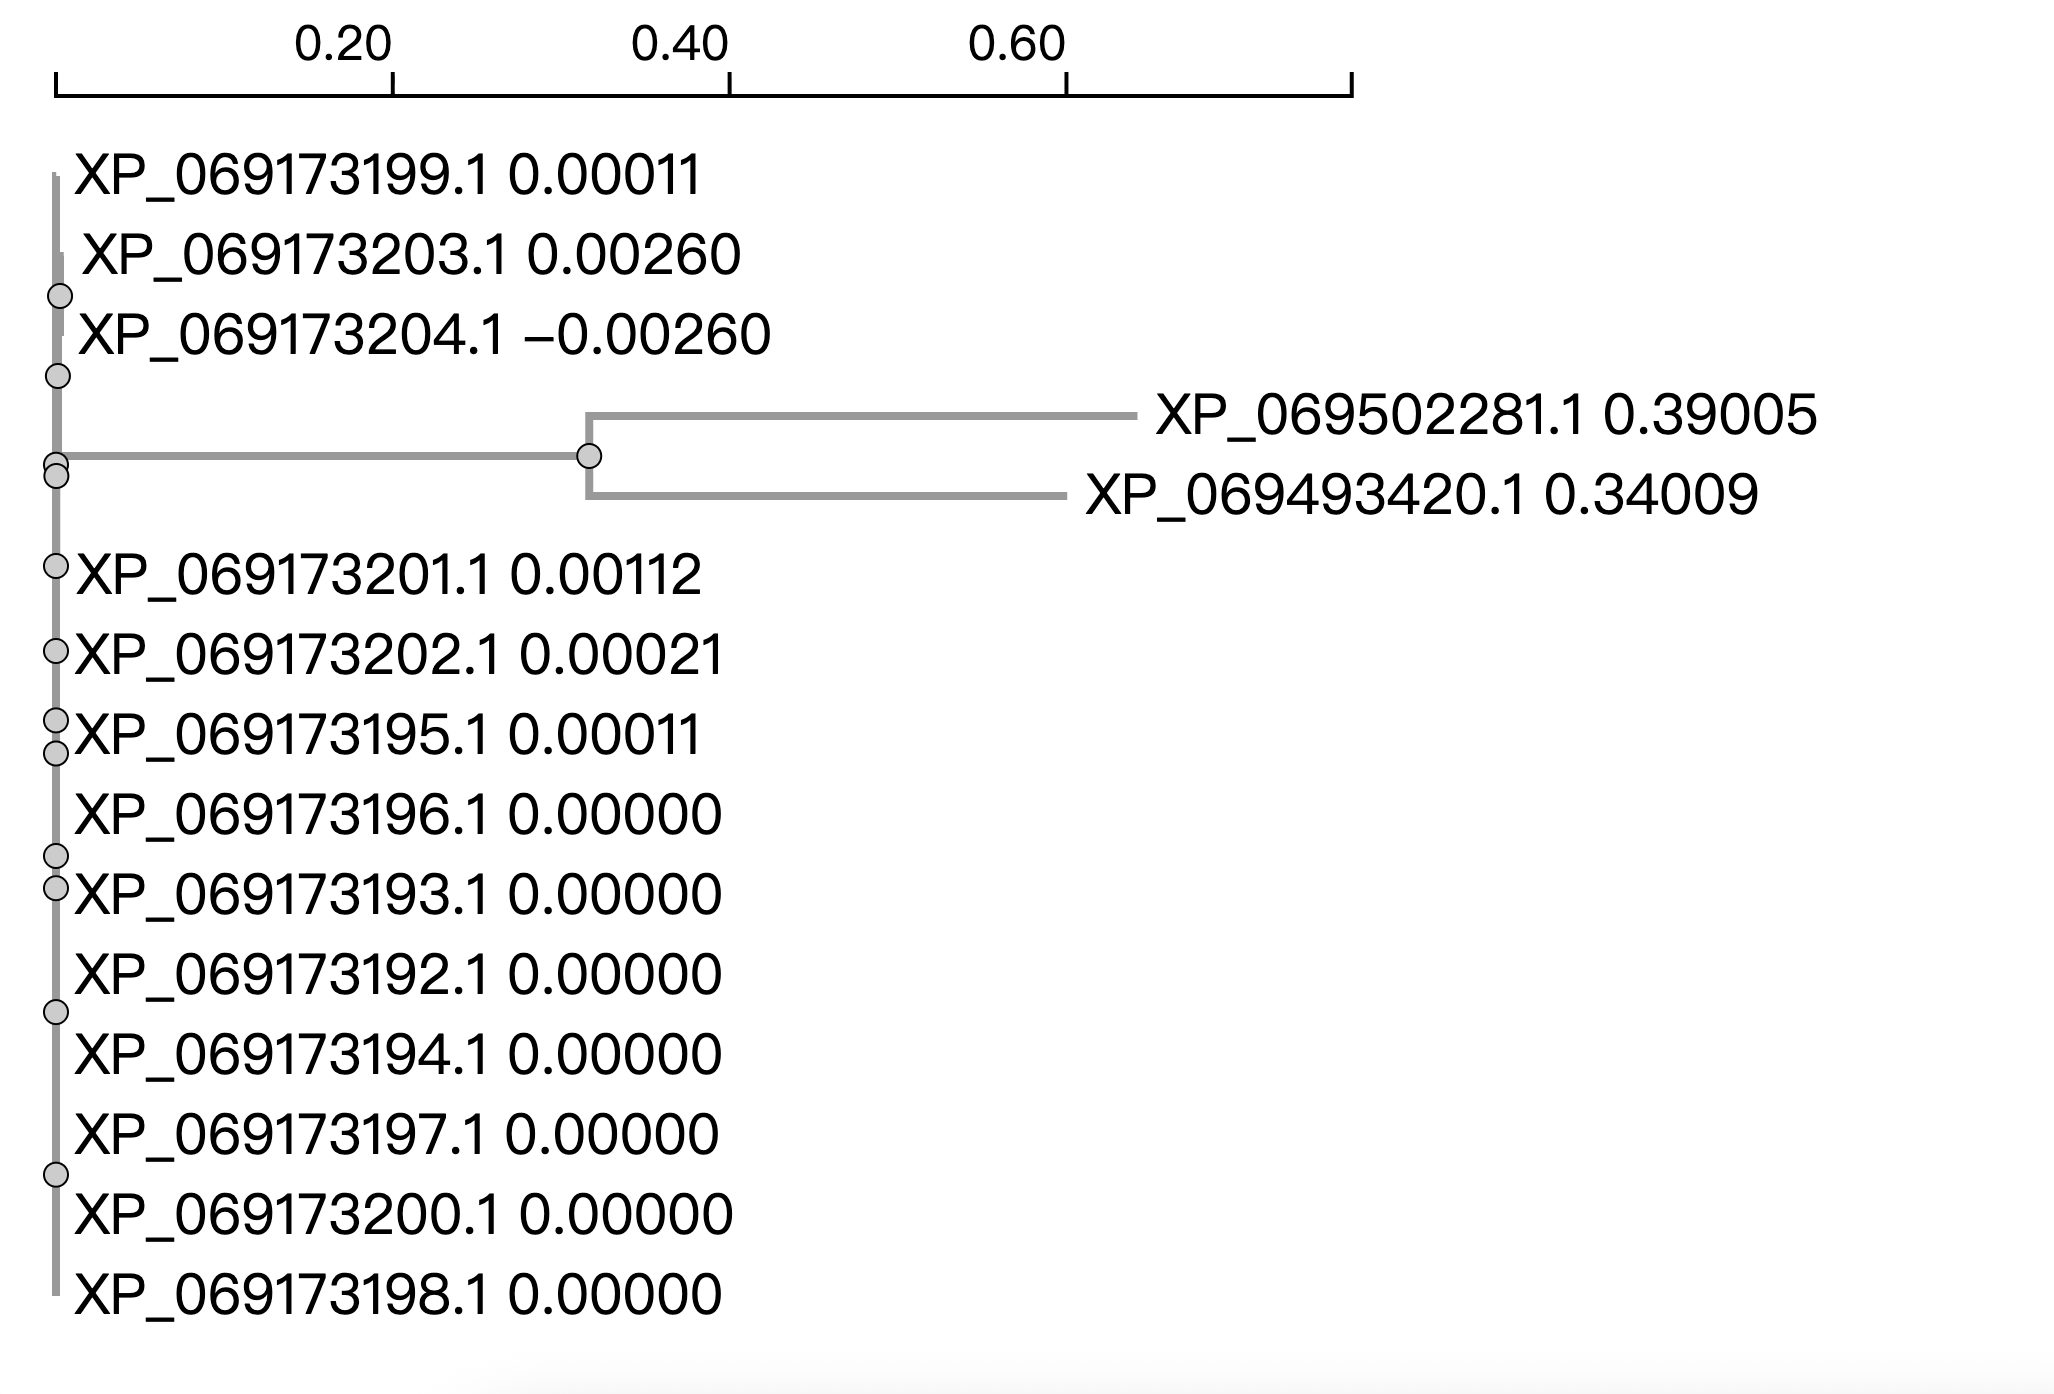
\includegraphics[width=0.8\textwidth]{image.png}
    \caption{Phylogenetic Tree}
    \label{fig:phylo-tree}
\end{figure}
